%beamer

% Comment/uncomment this line to toggle handout mode
\newcommand{\handout}{}

%% Beamer-Klasse im korrekten Modus
\ifdefined \handout
\documentclass[handout]{beamer} % Handout mode
\else
\documentclass{beamer}
\fi

%% UTF-8-Encoding
\usepackage[utf8]{inputenc}

\input{../framework/gbi-macros}
\usepackage[blue]{../framework/thwregex}
\usepackage{environ}
\usepackage{bm}
\usepackage{calc}
\usepackage{varwidth}
\usepackage{wasysym}
\usepackage{mathtools}


% Das ist der KIT-Stil
%\usepackage{../TutTexbib/beamerthemekit}
\usepackage[deutsch,titlepage0]{../framework/KIT/beamerthemeKITmod}
\TitleImage[width=\titleimagewd]{../figures/titlepage.jpg}
%\usetheme[deutsch,titlepage0]{KIT}

% Include PDFs
\usepackage{pdfpages}

% Libertine font (Original GBI font)
\usepackage{libertine}
%\renewcommand*\familydefault{\sfdefault}  %% Only if the base font of the document is to be sans serif

% Nicer math symbols
\usepackage{eulervm}
%\usepackage{mathpazo}
\renewcommand\ttdefault{cmtt} % Computer Modern typewriter font, see lecture slides.

\usepackage{csquotes}

%%%%%%

%% Schönere Schriften
\usepackage[TS1,T1]{fontenc}

%% Bibliothek für Graphiken
\usepackage{graphicx}

%% der wird sowieso in jeder Datei gesetzt
\graphicspath{{../figures/}}

%% Anzeigetiefe für Inhaltsverzeichnis: 1 Stufe
\setcounter{tocdepth}{1}

%% Hyperlinks
\usepackage{hyperref}
% I don't know why, but this works and only includes sections and NOT subsections in the pdf-bookmarks.
\hypersetup{bookmarksdepth=subsection} 

%\usepackage{lmodern}
\usepackage{colortbl}
\usepackage[absolute,overlay]{textpos}
\usepackage{listings}
\usepackage{forloop}
%\usepackage{algorithmic} % PseudoCode package 

\usepackage{tikz}
\usetikzlibrary{matrix}
\usetikzlibrary{arrows.meta}
\usetikzlibrary{automata}
\usetikzlibrary{tikzmark}
\usetikzlibrary{positioning}

% Why has no-one come up with this yet? I mean, seriously. -.-
\tikzstyle{loop below right} = [loop, out=-60,in=-30, looseness=7]
\tikzstyle{loop below left} = [loop, out=-150,in=-120, looseness=7]
\tikzstyle{loop above right} = [loop, out=60,in=30, looseness=7]
\tikzstyle{loop above left} = [loop, out=150,in=120, looseness=7]
\tikzstyle{loop right below} = [loop below right]
\tikzstyle{loop left below} = [loop below left]
\tikzstyle{loop right above} = [loop above right]
\tikzstyle{loop left above} = [loop above left]

% Needed for gbi-macros
\usepackage{xspace}

%%%%%%

%% Verbatim
\usepackage{moreverb}

%%%%%%%%%%%%%%%%%%%%%%%%%%%%%%%%%%%% Copy end

%% Tabellen
\usepackage{array}
\usepackage{multicol}
\usepackage{hhline}

%% Bibliotheken für viele mathematische Symbole
\usepackage{amsmath, amsfonts, amssymb}

%% Deutsche Silbentrennung und Beschriftungen
\usepackage[ngerman]{babel}

\usepackage{kbordermatrix}

% kbordermatrix settings
\renewcommand{\kbldelim}{(} % Left delimiter
\renewcommand{\kbrdelim}{)} % Right delimiter

\input{../config.tex}



% define custom \handout command flag if handout mode is toggled  #DirtyAsHellButWell...
\only<beamer:0>{\def\handout{}} %beamer:0 == handout mode

\newcommand{\R}{\mathbb{R}}
\newcommand{\N}{\mathbb{N}}
\newcommand{\Z}{\mathbb{Z}}
\newcommand{\Q}{\mathbb{Q}}
\newcommand{\BB}{\mathbb{B}}
\newcommand{\C}{\mathbb{C}}
\newcommand{\K}{\mathbb{K}}
\newcommand{\G}{\mathbb{G}}
\newcommand{\nullel}{\mathcal{O}}
\newcommand{\einsel}{\mathds{1}}
\newcommand{\Pot}{\mathcal{P}}
\renewcommand{\O}{\text{O}}

\def\word#1{\hbox{\textcolor{blue}{\texttt{#1}}}}
\let\literal\word
\def\mword#1{\hbox{\textcolor{blue}{$\mathtt{#1}$}}}  % math word
\def\sp{\scalebox{1}[.5]{\textvisiblespace}}
\def\wordsp{\word{\sp}}

%\newcommand{\literal}[1]{\textcolor{blue}{\texttt{#1}}}
\newcommand{\realTilde}{\textasciitilde \ }
\newcommand{\setsize}[1]{\ensuremath{\left\lvert #1 \right\rvert}}
\newcommand{\size}[1]{\setsize{#1}}  % Shame on you, TeXStudio...
\newcommand{\set}[1]{\left\{#1\right\}}
\newcommand{\tuple}[1]{\left(#1\right)}
\newcommand{\normalvar}[1]{\text{$#1$}}

% Modified by DJ
\let\oldemptyset\emptyset
\let\emptyset\varnothing % proper emptyset

\newcommand{\boder}{\ensuremath{\mathbin{\textcolor{blue}{\vee}}}\xspace}
\newcommand{\bund}{\ensuremath{\mathbin{\textcolor{blue}{\wedge}}}\xspace}
\newcommand{\bimp}{\ensuremath{\mathrel{\textcolor{blue}{\to}}}\xspace}
\newcommand{\bgdw}{\ensuremath{\mathrel{\textcolor{blue}{\leftrightarrow}}}\xspace}
\newcommand{\bnot}{\ensuremath{\textcolor{blue}{\neg}}\xspace}
\newcommand{\bone}{\ensuremath{\textcolor{blue}{1}}\text{}}
\newcommand{\bzero}{\ensuremath{\textcolor{blue}{0}}\text{}}
\newcommand{\bleftBr}{\ensuremath{\textcolor{blue}{\texttt{(}}}\text{}}
\newcommand{\brightBr}{\ensuremath{\textcolor{blue}{\texttt{)}}}\text{}}

% Fix of \b... commands:

\renewcommand{\boder}{\alor}
\renewcommand{\bund}{\aland}
\renewcommand{\bimp}{\alimpl}
\renewcommand{\bgdw}{\aleqv}
\renewcommand{\bnot}{\alnot}
\renewcommand{\bleftBr}{\alka}
\renewcommand{\brightBr}{\alkz}
\newcommand{\alA}{\word A}
\newcommand{\alB}{\word B}
\newcommand{\alC}{\word C}

\newcommand{\plB}{\plfoo{B}}
\newcommand{\plE}{\plfoo{E}}

\newcommand{\summe}[2]{\sum\limits_{#1}^{#2}}
\newcommand{\limes}[1]{\lim\limits_{#1}}

%\newcommand{\numpp}{\advance \value{weeknum} by -2 \theweeknum \advance \value{weeknum} by 2}
%\newcommand{\nump}{\advance \value{weeknum} by -1 \theweeknum \advance \value{weeknum} by 1}

\newcommand{\mycomment}[1]{}
\newcommand{\Comment}[1]{}

%% DISCLAIMER START 
% It is INSANELY IMPORTANT NOT TO DO THIS OUTSIDE BEAMER CLASS! IN ARTCILE DOCUMENTS, THIS IS VERY LIKELY TO BUG AROUND!
\makeatletter%
\@ifclassloaded{beamer}%
{
	% TODO 
	% no time... later.   (= never -.-)
	% redefine section to ignore multiple \section calls with the same title
}%
{
	\errmessage{ERROR: section command redefinition outside of beamer class document! Please contact the author of this code or read the F-ing disclaimer.}
}%
\makeatother%
%% DISCLAIMER END

\newcounter{abc}
\newenvironment{alist}{
  \begin{list}{(\alph{abc})}{
      \usecounter{abc}\setlength{\leftmargin}{8mm}\setlength{\labelsep}{2mm}
    }
}{\end{list}}


\newcommand{\stdarraystretch}{1.20}
\renewcommand{\arraystretch}{\stdarraystretch}  % for proper row spacing in tables

\newcommand{\morescalingdelimiters}{   % for proper \left( \right) typography
	\delimitershortfall=-1pt  
	\delimiterfactor=1
}

\newcommand{\centered}[1]{\vspace{-\baselineskip}\begin{center}#1\end{center}\vspace{-\baselineskip}}

% for \implitem and \item[bla] stuff to look right:
\setbeamercolor*{itemize item}{fg=black}
\setbeamercolor*{itemize subitem}{fg=black}
\setbeamercolor*{itemize subsubitem}{fg=black}

\setbeamercolor*{description item}{fg=black}
\setbeamercolor*{description subitem}{fg=black}
\setbeamercolor*{description subsubitem}{fg=black}

\renewcommand{\qedsymbol}{\textcolor{black}{\openbox}}

\renewcommand{\mod}{\mathop{\textbf{mod}}}
\renewcommand{\div}{\mathop{\textbf{div}}}

\newcommand{\ceil}[1]{\left\lceil#1\right\rceil}
\newcommand{\floor}[1]{\left\lfloor#1\right\rfloor}
\newcommand{\abs}[1]{\left\lvert #1 \right\rvert}
\newcommand{\Matrix}[1]{\begin{pmatrix} #1 \end{pmatrix}}
\newcommand{\braced}[1]{\left\lbrace #1 \right\rbrace}

% "something" placeholder. Useful for repairing spacing of operator sections, like `\sth = 42`.
\def\sth{\vphantom{.}}

\def\fract#1/#2 {\frac{#1}{#2}} % ! Trailing space is crucial!
\def\dfract#1/#2 {\dfrac{#1}{#2}} % ! Trailing space is crucial!

\newcommand{\Mid}{\;\middle|\;}

\let\after\circ



\def\·{\cdot}
\def\*{\cdot}
\def\?>{\ensuremath{\rightsquigarrow}}  % Fuck you, Latex
\def\~~>{\ensuremath{\rightsquigarrow}}  

\newcommand{\tight}[1]{{\renewcommand{\arraystretch}{0.76} #1}}
\newcommand{\stackedtight}[1]{\renewcommand{\arraystretch}{0.76} \begin{matrix} #1 \end{matrix} }
\newcommand{\stacked}[1]{\begin{matrix} #1 \end{matrix} }
\newcommand{\casesl}[1]{\delimitershortfall=0pt  \left\lbrace\hspace{-.3\baselineskip}\begin{array}{ll} #1 \end{array}\right.}
\newcommand{\casesr}[1]{\delimitershortfall=0pt  \left.\begin{array}{ll} #1 \end{array}\hspace{-.3\baselineskip}\right\rbrace}
\newcommand{\caseslr}[1]{\delimitershortfall=0pt  \left\lbrace\hspace{-.3\baselineskip}\begin{array}{ll} #1 \end{array}\hspace{-.3\baselineskip}\right\rbrace}

\def\q#1uad{\ifnum#1=0\relax\else\quad\q{\the\numexpr#1-1\relax}uad\fi}
% e.g. \q1uad = \quad, \q2uad = \qquad etc.

\newcommand{\qqquad}{\q3uad}
\newcommand{\minusquad}{\hspace{-1em}}

%% Placeholder utils
% \§{#1}   Saves #1 as placeholder and prints it
% \.       Prints an \hphantom with the size of the recalled placeholder.
\def\indentstring{}
\def\§#1{\def\indentstring{#1}#1}
\def\.{{$\hphantom{\text{\indentstring}}$}}
%% Placeholder utils end

\newcommand{\impl}{\ifmmode\ensuremath{\mskip\thinmuskip\Rightarrow\mskip\thinmuskip}\else$\Rightarrow$\fi\xspace}
\newcommand{\Impl}{\ifmmode\implies\else$\Longrightarrow$\fi\xspace}

\newcommand{\derives}{\Rightarrow}

\newcommand{\gdw}{\ifmmode\mskip\thickmuskip\Leftrightarrow\mskip\thickmuskip\else$\Leftrightarrow$\fi\xspace}
\newcommand{\Gdw}{\ifmmode\iff\else$\Longleftrightarrow$\fi\xspace}

% Legacy code from the algo tutorial slides. Perhaps useful. Try with care.
\mycomment{
	\newcommand{\impl}{\ifmmode\ensuremath{\mskip\thinmuskip\Rightarrow\mskip\thinmuskip}\else$\Rightarrow$\xspace\fi}  
	\newcommand{\Impl}{\ifmmode\implies\else$\Longrightarrow$\xspace\fi}
	
	\newcommand{\gdw}{\ifmmode\mskip\thickmuskip\Leftrightarrow\mskip\thickmuskip\else$\Leftrightarrow$\xspace\fi}
	\newcommand{\Gdw}{\ifmmode\iff\else$\Longleftrightarrow$\xspace\fi}
}
	
\newcommand{\gdwdef}{\ifmmode\mskip\thickmuskip:\Leftrightarrow\mskip\thickmuskip\else:$\Leftrightarrow$\xspace\fi}
\newcommand{\Gdwdef}{\ifmmode\mskip\thickmuskip:\Longleftrightarrow\mskip\thickmuskip\else:$\Longleftrightarrow$\xspace\fi}

\newcommand{\symbitemnegoffset}{\hspace{-.5\baselineskip}}
\newcommand{\implitem}{\item[\impl\symbitemnegoffset]}
\newcommand{\Implitem}{\item[\Impl\symbitemnegoffset]}


\newcommand{\forcenewline}{\mbox{}\\}

\newcommand{\bfalert}[1]{\textbf{\alert{#1}}}
\let\elem\in   % I'm a Haskell freak. Don't judge me. :P


\def\|#1|{\text{\normalfont #1}}  % | steht für senkrecht (anstatt kursiv wie sonst im math mode)


% proper math typography
\newcommand{\functionto}{\longrightarrow}
\renewcommand{\geq}{\geqslant}
\renewcommand{\leq}{\leqslant}
\let\oldsubset\subset
\renewcommand{\subset}{\subseteq} % for all idiots out there using subset

\newenvironment{threealign}{%
	\[
	\begin{array}{r@{\ }c@{\ }l}
}{%
	\end{array}	
	\]
}

\newcommand{\concludes}{ \\ \hline  }
\newcommand{\deduction}[1]{
	\begin{varwidth}{.8\linewidth}
		\begin{tabular}{>{$}c<{$}}
			#1
		\end{tabular}
	\end{varwidth}	
}

\definecolor{hoareorange}{rgb}{1,.85,.6}
\newcommand{\hoareassert}[1]{\setlength{\fboxsep}{1pt}\setlength{\fboxrule}{-1.4pt}\fcolorbox{white}{hoareorange}{\ensuremath{\{\;#1\;\}}}\setlength\fboxrule{\defaultfboxrule}\setlength{\fboxsep}{3pt}}

\newcommand{\mailto}[1]{\href{mailto:#1}{{\textcolor{blue}{\underline{#1}}}}}
\newcommand{\urlnamed}[2]{\href{#2}{\textcolor{blue}{\underline{#1}}}}
\renewcommand{\url}[1]{\urlnamed{#1}{#1}}

\newcommand{\hanging}{\hangindent=0.7cm}
\newcommand{\indented}{\hanging}


% \hstretchto prints #2 left-aligned into a box of the width of #1
\def\hstretchto#1#2{%
	\mbox{}\vphantom{#2}\rlap{#2}\hphantom{#1}%
}

\def\vstretchto#1#2{%
	\mbox{}\hphantom{#2}\smash{#2}\vphantom{#1}%
}

% \hstretchtocentered prints #2 centered into a box of the width of #1
\def\hstretchtocentered#1#2{%
	\mbox{}\vphantom{#2}\scalebox{0.5}{\hphantom{#1}}\clap{#2}\scalebox{0.5}{\hphantom{#1}}%
}

% vertical centering
\newcommand{\vertcenter}[1]{%
	\ensuremath{\vcenter{\hbox{#1}}}%
}


%requires \thisyear to be defined (s. config.tex)!
\edef\nextyear{\the\numexpr\thisyear+1\relax}


% --- \frameheight constant ---
\newlength\fullframeheight
\newlength\framewithtitleheight
\setlength\fullframeheight{.92\textheight}
\setlength\framewithtitleheight{.86\textheight}

\newlength\frameheight
\setlength\frameheight{\fullframeheight}

\let\frametitleentry\relax
\let\oldframetitle\frametitle
\def\newframetitle#1{\global\def\frametitleentry{#1}\if\relax\frametitleentry\relax\else\setlength\frameheight{\framewithtitleheight}\fi\oldframetitle{#1}}
\let\frametitle\newframetitle

\def\newframetitleoff{\let\frametitle\oldframetitle}
\def\newframetitleon{\let\frametitle\newframetitle}
% --- \frameheight constant end ---

\newcommand{\fakeframetitle}[1]{%
	\vspace{-2.05\baselineskip}%
	{\Large \textbf{#1}} \\%
	\smallskip
}



\newenvironment{headframe}{\Huge THIS IS AN ERROR. PLEASE CONTACT THE ADMIN OF THIS TEX CODE. (headframe env def failed)}{}
\RenewEnviron{headframe}[1][]{
	\begin{frame}\frametitle{\ }
		\centering
		\Huge\textbf{\textsc{\BODY} \\
		}
		\Large {#1}
		\frametitle{\ }
	\end{frame}
}


\makeatletter
% Provides color if undefined.
\newcommand{\colorprovide}[2]{%
	\@ifundefinedcolor{#1}{\colorlet{#1}{#2}}{}}
\makeatother


\colorprovide{lightred}{red!30}
\colorprovide{lightgreen}{green!40}
\colorprovide{lightyellow}{yellow!50}
\colorprovide{lightblue}{blue!10}
\colorprovide{beamerlightred}{lightred}
\colorprovide{beamerlightgreen}{lightgreen}
\colorprovide{beamerlightyellow}{lightyellow}
\colorprovide{beamerlightblue}{lightblue}
\colorprovide{fullred}{red!60}
\colorprovide{fullgreen}{green}
\definecolor{darkred}{RGB}{115,48,38}
\definecolor{darkgreen}{RGB}{48,115,38}
\definecolor{darkyellow}{RGB}{100,100,0}

\only<handout:0>{\colorlet{adaptinglightred}{beamerlightred}}
\only<handout:0>{\colorlet{adaptinglightgreen}{beamerlightgreen}}
\only<handout:0>{\colorlet{adaptinglightyellow}{beamerlightyellow}}
\only<handout:0>{\colorlet{adaptinglightblue}{beamerlightblue}}
\only<beamer:0>{\colorlet{adaptinglightred}{lightred}}
\only<beamer:0>{\colorlet{adaptinglightgreen}{lightgreen}}
\only<beamer:0>{\colorlet{adaptinglightyellow}{lightyellow}}
\only<beamer:0>{\colorlet{adaptinglightblue}{lightblue}}
\only<handout:0>{\colorlet{adaptingred}{lightred}}
\only<beamer:0>{\colorlet{adaptingred}{fullred}}
\only<handout:0>{\colorlet{adaptinggreen}{lightgreen}}
\only<beamer:0>{\colorlet{adaptinggreen}{fullgreen}}



\newcommand{\TrueQuestion}[1]{
	\TrueQuestionE{#1}{}
}

\newcommand{\YesQuestion}[1]{
	\YesQuestionE{#1}{}
}

\newcommand{\FalseQuestion}[1]{
	\FalseQuestionE{#1}{}
}

\newcommand{\NoQuestion}[1]{
	\NoQuestionE{#1}{}
}

\newcommand{\DependsQuestion}[1]{
	\DependsQuestionE{#1}{}
}

\newcommand{\QuestionVspace}{\vspace{4pt}}
\newcommand{\QuestionParbox}[1]{\begin{varwidth}{.85\linewidth}#1\end{varwidth}}
\newcommand{\ExplanationParbox}[1]{\begin{varwidth}{.97\linewidth}#1\end{varwidth}}
\colorlet{questionlightgray}{gray!23}
\let\defaultfboxrule\fboxrule

% #1: bg color
% #2: fg color short answer
% #3: short answer text
% #4: question
% #5: explanation
\newcommand{\GenericQuestion}[5]{
	\setlength\fboxrule{2pt}
	\only<+|handout:0>{\hspace{-2pt}\fcolorbox{white}{questionlightgray}{\QuestionParbox{#4} \quad\textbf{?}}}
	\visible<+->{\hspace{-2pt}\fcolorbox{white}{#1}{\QuestionParbox{#4} \quad\textbf{\textcolor{#2}{#3}}} \if\relax#5\relax\else\ExplanationParbox{#5}\fi} \\
	\setlength\fboxrule{\defaultfboxrule}
}

% #1: Q text
% #2: Explanation
\newcommand{\TrueQuestionE}[2]{
	\GenericQuestion{adaptinglightgreen}{darkgreen}{Wahr.}{#1}{#2}
}

% #1: Q text
% #2: Explanation
\newcommand{\YesQuestionE}[2]{
	\GenericQuestion{adaptinglightgreen}{darkgreen}{Ja.}{#1}{#2}
}

% #1: Q text
% #2: Explanation
\newcommand{\FalseQuestionE}[2]{
	\GenericQuestion{adaptinglightred}{darkred}{Falsch.}{#1}{#2}
}

% #1: Q text
% #2: Explanation
\newcommand{\NoQuestionE}[2]{
	\GenericQuestion{adaptinglightred}{darkred}{Nein.}{#1}{#2}
}

% #1: Q text
% #2: Explanation
\newcommand{\DependsQuestionE}[2]{
	\GenericQuestion{adaptinglightyellow}{darkyellow}{Je nachdem!}{#1}{#2}
}

% #1: Q text
% #2: Answer
\newcommand{\ContentQuestion}[2]{
	\GenericQuestion{adaptinglightblue}{black}{\minusquad}{#1}{#2}
}

\ifnum\thisyear=2021 \else \errmessage{Old ILIAS link inside preamble. Please update.} \fi

\newcommand{\ILIAS}{\urlnamed{ILIAS}{\myILIASurl}\xspace}
\newcommand{\Klausurtermin}{\myKlausurtermin\xspace}

\newcommand{\Socrative}{\ifdefined\mysocrativeroom \only<handout:0>{socrative.com $\quad \~~> \quad $ Student login \\ Raumname:  \mysocrativeroom\\ \medskip}\else\fi}

\newcommand{\thasse}[1]{
	\ifdefined\ThassesTut #1\xspace \else\fi
}
\newcommand{\daniel}[1]{
	\ifdefined\DanielsTut #1\xspace \else\fi
}
\newcommand{\thassedaniel}[2]{\ifdefined\ThassesTut #1\else\ifdefined\DanielsTut #2\fi\fi\xspace}

\ifdefined\ThassesTut \ifdefined\DanielsTut \errmessage{ERROR: Both ThassesTut and DanielsTut flags are set. This is most likely an error. Please check your config.tex file.} \else \fi \else \ifdefined\DanielsTut \else \errmessage{ERROR: Neither ThassesTut  nor DanielsTut flags are set. This is most likely an error. Please check your config.tex file.} \fi\fi

%\newcommand{\sgn}{\text{sgn}}

%%%%%%%%%%%% INHALT %%%%%%%%%%%%%%%%

%% Wochennummer
\newcounter{weeknum}

%% Titelinformationen
\title[GBI-Tutorium \mytutnumber, Woche \theweeknum]{Grundbegriffe der Informatik \\ Tutorium \mytutnumber}

\subtitle{Woche \theweeknum\xspace |\xspace\mydate{\theweeknum} \\ \myname \ \  \normalfont (\mailto{\mymail})}
\author[\myname]{\myname}
\institute{KIT -- Karlsruher Institut für Technologie}
\date{\mydate{\theweeknum}\ }

% Modified, DJ (better safe than sorry)
\AuthorTitleSep{ – }

%% Titel einfügen
\newcommand{\titleframe}{\frame{\titlepage}}

%% Alles starten mit \starttut{X}
\newcommand{\starttut}[1]{\setcounter{weeknum}{#1}\pdfinfo{
		/Author (\myname)
		/Title  (GBI-Tutorium \mytutnumber, Woche \theweeknum)
	}\titleframe\frame{\frametitle{Inhalt}\tableofcontents} \AtBeginSection[]{%
		\begin{frame}{Wo sind wir gerade?}
		\tableofcontents[currentsection]
	\end{frame}\addtocounter{framenumber}{-1}}}


\newcommand{\framePrevEpisode}{
\begin{headframe}
	\mylasttimestext
\end{headframe}
}

\newcommand{\lastframetitled}[6]{
	\frame{\frametitle{#6}
		\vspace{-#2\baselineskip}
		\begin{figure}[H]
			\centering
			\LARGE \textbf{\textsc{#5}} \\
			\vspace{.2\baselineskip}
			\includegraphics[#1]{#3}
			\vspace{-6pt}
			\begin{center}
				\small \url{#4} 
			\end{center}
		\end{figure} 
	}
}

% #1 number
% #2 title 
% #3 vspace (positive) without unit (\baselineskip)
\newcommand{\xkcdframe}[3]{
	\lastframetitled{width=.96\textwidth}{#3}{xkcd/#1}{http://xkcd.com/#1}{}{#2}
}

\newcommand{\xkcdframevert}[3]
{
	\lastframetitled{height=.96\frameheight}{#3}{xkcd/#1}{http://xkcd.com/#1}{}{#2}
}

% #1 number
% #2 title 
% #3 vspace (positive) without unit (\baselineskip)
% #4 \includegraphics[] optional parameters
\newcommand{\xkcdframecustom}[4]
{
	\lastframetitled{#4}{#3}{xkcd/#1}{http://xkcd.com/#1}{}{#2}
}

\newcommand{\slideThanks}{
	\begin{frame}
	\frametitle{Credits}
	\begin{block}{}
		An der Erstellung des Foliensatzes haben mitgewirkt:\\[1em]
		Daniel Jungkind \\
		Thassilo Helmold \\
		Philipp Basler \\
		Nils Braun \\
		Dominik Doerner \\
		Ou Yue \\
		Max Schweikart
	\end{block}
\end{frame}
}

%% Wörter DEPRECATED! DO NOT USE
\newcommand{\code}[1]{$\mathbf{#1}$}

\morescalingdelimiters

\begin{document}
\starttut{13}

\section{Rückblick}

\begin{frame}{Zu Übungsblatt \#11}
	Bisheriger Schnitt: \quad 12.7 / 21~P

	\begin{itemize}
		\item 13 von 23 Tutanden haben etwas abgegeben
		\item Die Korrektur und die Musterlösung findet ihr wie immer im ILIAS-Aufgaben-Objekt
		\item Wenn ihr Fragen habt, meldet euch bei mir
	\end{itemize}
\end{frame}

\begin{frame}{Zu Übungsblatt \#11}
	Die häufigsten Fehler:
	\begin{itemize}[<+->]
		\item[1d)] ``Wie viele Knoten dürfen \textit{höchstens} in $F$ sein, damit ...''
		\implitem Begründen, warum für $|F| = 2$ nicht immer ein sicherer Weg existiert \textbf{und} dass für $|F|=1$ immer ein sicherer Weg existiert.
		\item[3)] Aussagen im O-Kalkül begründet man mit den \textit{Rechenregeln aus der Vorlesung} oder anhand der \textit{Definitionen von asymptotischen Wachstum}.
		\item Dabei \textbf{präzise} sein, z.B.: $2^{\sqrt{n}}$ hat nicht die Form ``$a^n$ für ein $a\in \mathbb{R}^+$''.
		\item $f_1 \preceq f_2$ bedeutet nicht unbedingt $f_2 \not\preceq f_1$
		\item \textbf{Auf keinen Fall} $f=\Oh{g}$ schreiben! $\Oh{g}$ ist eine Menge von Funktionen und man schreibt $f\in\Oh{g}$
		\item[*)] ``Laut Tutorium'' ist keine gute Begründung \smiley
	\end{itemize}
\end{frame}

\begin{frame}{Schwarzes Brett}
	\begin{itemize}
		\item Korrektur: Ein zusammenhängender ungerichteter Graph ist genau dann ein Baum, wenn es in ihm keine echten Kreise \textit{und keine Schleifen} gibt.
		\item Anmeldung \textbf{Klausur} $+$ \textbf{Übungsschein} nicht vergessen!
		\item Erinnerung: Klausur am \Klausurtermin
		\item Bonus: Übungsstunde am 22. Februar 2021, 12:00 - 13:30 Uhr
	\end{itemize}
\end{frame}

\framePrevEpisode

\begin{frame}{Kahoot!}
	\begin{itemize}[<+->]
		\item Kahoot! ist ein anonymes Online-Quiz
		\item Ihr bekommt Punkte für schnelles und richtiges raten
		\item Ihr könnt mit eurem Handy oder PC über \url{https://kahoot.it} mitspielen
		\item Das Kahoot! könnt ihr euch später nochmal unter diesem Link angucken: \\
			\url{https://create.kahoot.it/share/gbi-woche-13-einstieg/9cfc29f7-2261-49ce-974b-9ca3b305c81b}
	\end{itemize}
\end{frame}

%\begin{frame}[t]{Wahr oder Falsch?}
%	\FalseQuestionE{Das (komplizierte) Master-Theorem kann man immer anwenden.}{ Nur bei rekursiven Algorithmen, bei denen das Problem in gleich große Teilprobleme aufgeteilt wird.}
%	\FalseQuestionE{Jeder Moore-Automat kann in einen Mealy-Automaten umgewandelt werden, der für jedes Wort die gleiche Ausgabe produziert.}{ Für das leere Wort kann ein Mealy-Automat niemals eine Ausgabe produzieren.}
%	\TrueQuestionE{Endliche Akzeptoren sind Moore-Automaten mit dem Ausgabealphabet $\{\word 0,\word 1\}$.}{}
%	\FalseQuestionE{Mit endlichen Automaten kann jede beliebige Sprache erkannt \\ werden.}{Tatsächlich ist die Menge der akzeptierbaren Sprachen sogar sehr eingeschränkt.}	
%\end{frame}

\section{Endliche Akzeptoren}
\begin{frame}[t]{Endliche Akzeptoren}
	\begin{Definition}
		Ein \textbf{endlicher Akzeptor} $A$ ist ein \emph{Moore}-Automat mit Ausgabealphabet $ Y= \{\word 0,\word 1\}$, der zuletzt $\word 1$ ausgibt, falls ihm das Wort gefällt und \word 0 sonst.
	\end{Definition} 
	
	$A$ \textbf{akzeptiert} ein Wort $w$, wenn er als Letztes eine $\word 1$ ausgibt. \\ \medskip 
	
	\only<all:2>{
		\begin{center}
					\begin{tikzpicture}[->,>=stealth,shorten >=1pt,auto,node distance=1.8cm,
				semithick,initial text={}]
				\tikzstyle{every state}=[]
				
				\node[state] (A)                    {$a\io\word 0$};
				\node[state] (B) [right of=A] 	    {$b\io\word 1$};
				
				\end{tikzpicture}
		\end{center}
	}
	\only<all:3>{
		\begin{center}
					\begin{tikzpicture}[->,>=stealth,shorten >=1pt,auto,node distance=1.8cm,
				semithick,initial text={}]
				\tikzstyle{every state}=[]
				
				\node[state] (A)                    {$a$};
				\node[state, accepting] (B) [right of=A] {$b$};
				
				\end{tikzpicture}
		\end{center} 
		\emph{Notation:} Wir nennen die Menge der \textbf{akzeptierenden Zustände} $F$ und malen solche mit einem Doppelkreis. \\ 
	}
\end{frame}

\begin{frame}{Von einem Akzeptor erkannte Sprache}
	Wir sprechen von einer \textbf{akzeptierten Sprache} über einem Alphabet. Sie ist definiert als 
	\begin{align*}
		L(A) &:= \{ w \mid f_*(z_0,w) \in F \}  \\
			 &\: = \{ w \mid g_*(z_0,w) = \word 1 \}.
	\end{align*}
	Also sind in einer akzeptierten Sprache alle Wörter, die von $A$ akzeptiert werden. \pause
	
	\begin{Beispiel}
		Sei $A$ gegeben als
		\vspace{-2\baselineskip}
		\begin{center}
			\begin{tikzpicture}[->,>=stealth,shorten >=1pt,auto,node distance=1.8cm,
			semithick,initial text={}]
			\tikzstyle{every state}=[]
			
			\node[initial, state, accepting] (A)                    {$z_0$};
			\node[state] (B) [right of=A] {$z_1$};
			
			\path
				(A) edge [loop above] node {\word a, \word b}  (A)
					edge [bend right=7] node [below] {\word c} 		  (B)
				(B) edge [loop right] node {\word c}		  (B)
					edge [bend right=7] node [above] {\word a, \word b} (A)
			;
			\end{tikzpicture}. % Sätze enden mit nem Punkt! :D
		\end{center} 
		\pause
		Dann ist $L(A) = \set{w \in \set{\word a, \word b, \word c}^* \Mid \text{$w$ endet nicht auf \word c}}$.
	\end{Beispiel}
\end{frame}

\begin{frame}{Aufgaben}
	Gebt einen Akzeptor an, der die Sprache aller Binärzahlen erkennt, die Zweierpotenzen darstellen. 
	\pause ($= \set{\word 0}^* \* \set{\word 1} \* \set{\word 0}^*$) \\
	%\vspace{-2\baselineskip}
	\begin{center}
		\begin{tikzpicture}[->,>=stealth,shorten >=1pt,auto,node distance=2cm,
		semithick,initial text={}]
		\tikzstyle{every state}=[]
		
		\node[initial,state] (A)                    {$a$};
		\node[state,accepting] (B)  [right of=A]     {$b$};
		\node[state]		 (M)  [right of=B]		{$m$};
		
		\path
		(A) edge [loop above]  node {\word 0} (A) 
		(A) edge 			  node {\word 1} (B) 
		(B) edge [loop above]  node {\word 0} (B) 
		(B) edge 			  node {\word 1} (M) 
		(M) edge [loop above] node {\word 0, \word 1} (M);
		\end{tikzpicture}
	\end{center}
	\pause
	\begin{block}{Bonusaufgabe}
		Gebt einen Akzeptor an, der die Sprache aller geraden Binärzahlen erkennt. 
		\pause ($= \set{\word 0,\word 1}^* \* \set{\word 0}$) \\
		%\vspace{-2\baselineskip}
		\begin{center}
			\begin{tikzpicture}[->,>=stealth,shorten >=1pt,auto,node distance=1.8cm,
			semithick,initial text={}]
			\tikzstyle{every state}=[]
			
			\node[initial, state] (A)                    {$a$};
			\node[state, accepting] (B) [right of=A] {$b$};
			
			\path
			(B) edge [loop above] node  {\word 0}  (B)
				edge [bend right=7] node [above] {\word 1} 		  (A)
			(A) edge [loop above] node  {\word 1}		  (A)
				edge [bend right=7] node [below] {\word 0} (B)
			;
			\end{tikzpicture}
		\end{center} 
	\end{block}
\end{frame}

\begin{frame}{Aufgabe}
	Der endliche Akzeptor $A = (Z, z_0, X, f, F)$ sei gegeben durch
	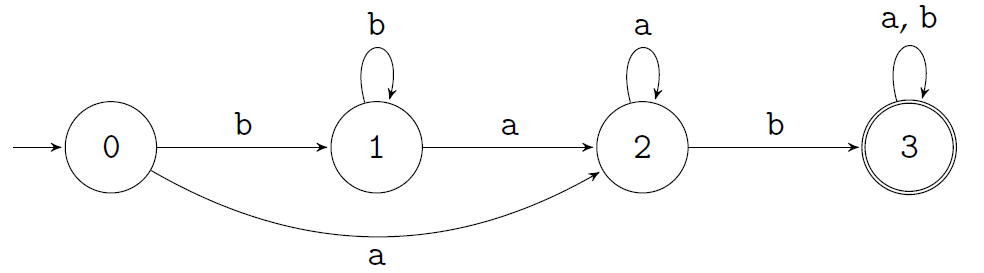
\includegraphics[scale=0.4]{automaten/akz1516B12A1}
	
	Gebt die von $A$ akzeptierte Sprache $L(A)$ unter ausschließlicher Benutzung der formalen Sprachen $\{\word a\}$, $\{\word b\}$, sowie $\{\word a, \word b\}$, des Konkatenationsabschlusses und des Produkts formaler Sprachen an.
	
	\emph{Beispiel:} $\{\word a, \word b\}^* \cdot \{\word a\} \cdot \{\word b\}$
	
	\visible<2-|handout:2>{
		\begin{block}{Lösung}
			$L(A) = \{\word b\}^* \cdot \{\word a\} \cdot \{\word a\}^* \cdot \{\word b\} \cdot \{\word a, \word b\}^*$ \\
			$\hphantom{L(A) } = \{\word b\}^* \cdot \hphantom{\{\word a\} \cdot \mbox{}} \{\word a\}^+ \!\cdot \{\word b\} \cdot \{\word a, \word b\}^*$
		\end{block}
	}
\end{frame}

\begin{frame}{Bonusaufgabe}
	\begin{enumerate}[a)]
		\item Zeichnet einen möglichst kleinen endlichen Akzeptor mit $ X = \{\word a, \word b\}$, der alle Wörter akzeptiert, bei denen die Anzahl der $\word a$ durch $5$ teilbar ist.
		\item Zeichnet einen Akzeptor mit $ X = \{\word a,\word b\}$, der alle Wörter akzeptiert, in denen nirgends hintereinander zwei $\word b$ vorkommen.
	\end{enumerate}		
\end{frame}

\begin{frame} {Lösung Bonusaufgabe a)}
	\begin{figure}[H] 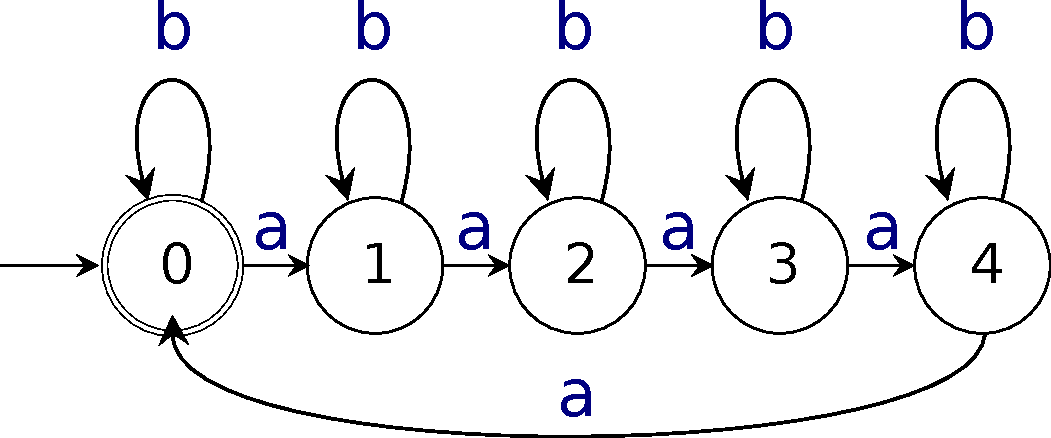
\includegraphics[scale=0.5]{automaten/Akzeptor1.pdf} \end{figure}		
\end{frame} 

\begin{frame}{Lösung Bonusaufgabe b)}
	\begin{figure}[H] 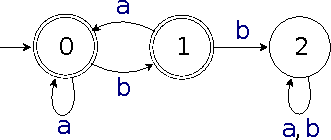
\includegraphics[scale=1.5]{automaten/Akzeptor2.pdf} \end{figure}
\end{frame}



\graphicspath{{../figures/}}

\newenvironment{Messtabelle}[1]
{\begin{minipage}{\linewidth} \centering  \begin{tabular}{#1} }
{\end{tabular} \vspace*{1em} \end{minipage}} 

\section{Turingmaschinen}

\begin{frame}{Grenzen endlicher Automaten}
	Automaten sind uns nicht mächtig genug:
	\begin{itemize}[<+->]
		\item sie können nicht ``zählen''
		\item Beispiel: $L=\left\{ w \in \left\{ \word a, \word b \right\}^* \text{ | } w \text{ enthält genau so viele \word as wie \word bs } \right\}$ kann nicht erkannt werden
		\item im Zustand können nur endlich viele Informationen kodiert werden
		\implitem zusätzlichen, unbegrenzten Speicher hinzufügen
		\implitem Automat mit \textbf{Band}: die Turingmaschine
	\end{itemize}
\end{frame}

\subsection{Inhalt}
\mycomment{ % no time
\begin{frame}{Turingmaschine}
	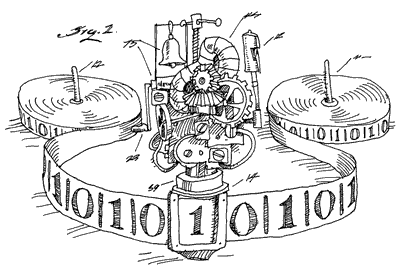
\includegraphics[scale=1]{turing/tmAufbau}
\end{frame}

% Kann ich erst Werbung für machen, nachdem ich ihn selbst gesehen habe, sonst wird's unglaubwürdig... :P
% Dann solltest du ihn unbedingt mal anschauen!
\thasse{
	\begin{frame}{Alan Turing}
		\centering
		\vspace{-25pt}
		
\includegraphics[scale=0.35]{turing/imitationGame}
	\end{frame}
}
} % end mycomment

%Das hier am Besten hinmalen mit Band und Schreiblesekopf und an der Tafel machen:
\begin{frame}{Eine einfache Turingmaschine}
	\begin{center}
		\begin{tikzpicture}[->,>=stealth,shorten >=1pt,auto,node distance=2.8cm,
		semithick,initial text={}]
		\tikzstyle{every state}=[]
		
		\node[initial,state] (A)                    {$a$};
		\node[state]         (M) [right of=A] 	    {$m$};
		
		\path 
		(A) edge [loop above] node {$\word 1\io\word 0R$} (A)
		edge [loop below]  node {$\word 0\io\word 1R$} (A)
		edge 					  node {$\word{2}\io\word{X}R$} (M)
		(M) edge [loop right] node {$\stackedtight{\word 0\io\word XR \\ \word 1\io\word XR \\ \word 2\io\word XR}$} (M)
		;
		\end{tikzpicture}
	\end{center} \pause
	Diese TM vertauscht $\word 1$en und $\word 0$en und ist beleidigt, wenn sie eine $\word 2$ liest. \\ \pause
	\begin{tabular}{rl@{\ \?>\ }rl}
		Zustand vorher: & a &  nachher: & \hphantom{\word{100010}}a \\
		Band vorher: &\word{011101} &  nachher:&  \word{100010}$\9$\\
		\hline
		Zustand vorher: & a &  nachher: & \hphantom{\word{100010}}m \\
		Band vorher: &\word{011102} &  nachher:&  \word{10001X}$\9$\\
		\hline
		Zustand vorher: & a &  nachher: & \hphantom{\word{100010}}m \\
		Band vorher: &\word{012101} &  nachher:&  \word{10XXXX}$\9$\\
	\end{tabular}

\end{frame}



\begin{frame}{Turingmaschinen}
	Eine Turingmaschine besteht aus...
	\begin{itemize}[<+->]
		\item einem unendlichen Band mit einzelnen Zellen, in denen jeweils genau ein Symbol aus dem Bandalphabet steht
		\item einem Schreib-/Lesekopf, der auf genau einer Bandzelle steht
		\item einer Steuerungseinheit (ähnlich zu einem Moore-Automat, mit der Ausgabe in den Übergängen), die sich in genau einem Zustand befindet
	\end{itemize}
\end{frame}

\begin{frame}{Funktionsweise der TM}
	In jedem Ausführungsschritt:
	\begin{itemize}[<+->]
		\item TM liest das Symbol, auf dem der Kopf steht
		\item Steuerung entscheidet über die Ausgabe, den Folgezustand und die Bewegung
		\item Ausgabe wird an der aktuellen Position auf das Band geschrieben
		\item Steuerung wechselt in den Folgezustand
		\item Kopf bewegt sich einen Schritt nach links (L) oder rechts (R) oder bleibt stehen (0)
	\end{itemize}
	\pause
	Die TM \textbf{hält}, wenn für einen Zustand und das gelesene Symbol keine Übergänge in der Steuerung definiert sind. \textbf{Eine TM muss nicht halten!} \\
	\impl Es können „Pfeile fehlen“!
\end{frame}

\begin{frame}{Eine einfache Turingmaschine v2}
	\begin{center}
		\begin{tikzpicture}[->,>=stealth,shorten >=1pt,auto,node distance=2.8cm,
		semithick,initial text={}]
		\tikzstyle{every state}=[]
		
		\node[initial,state] (A)                    {$a$};
		
		\path 
		(A) edge [loop above] node {$\word 1\io\word 0R$} (A)
		edge [loop below]  node {$\word 0\io\word 1R$} (A)
		;
		\end{tikzpicture}
	\end{center} \pause
	Pfeil für Eingabe \word 2 fehlt jetzt! \pause \impl TM hört dann einfach auf! \\ \pause
	\begin{tabular}{rl@{\ \?>\ }rl}
		Zustand vorher: & a &  nachher: & \hphantom{\word{100010}}a \\
		Band vorher: &\word{011101} &  nachher:&  \word{100010}$\9$\\
		\hline
		Zustand vorher: & a &  nachher: & \hphantom{\word{10001}}a \\
		Band vorher: &\word{011102} &  nachher:&  \word{100012}\\
		\hline
		Zustand vorher: & a &  nachher: & \hphantom{\word{10}}a \\
		Band vorher: &\word{012101} &  nachher:&  \word{102101}\\
	\end{tabular}
	
\end{frame}

\begin{frame}{Eine einfache Turingmaschine, Rage-Mode!}
	\begin{center}
		\begin{tikzpicture}[->,>=stealth,shorten >=1pt,auto,node distance=2.8cm,
		semithick,initial text={}]
		\tikzstyle{every state}=[]
		
		\node[initial,state] (A)                    {$a$};
		\node[state]         (M) [right of=A] 	    {$m_1$};
		\node[state]         (M2) [right of=M] 	    {$m_2$};
		
		\path 
		(A) edge [loop above] node {$\stackedtight{\word 1\io\word 0R \\ \word 0\io\word 1R}$} (A)
		edge 					  node {$\word{2}\io\word{2}R$} (M)
		(M) edge [loop above] node {$\stackedtight{\word 0\io\word 0R \\ \word 1\io\word 1R \\ \word 2\io\word 2R}$} (M)
		edge 					  node {$\9\io\9L$} (M2)
		(M2) edge [loop right] node {$\stackedtight{\word 0\io\9L \\ \word 1\io\9L \\ \word 2\io\9L}$} (M2)
		;
		\end{tikzpicture}
	\end{center} \pause
	\impl Löscht das komplette Eingabewort, wenn sie ne \word 2 in die Finger kriegt! \smiley \\ \pause
	\begin{tabular}{rl@{\ \?>\ }rl}
		Zustand vorher: & a &  nachher: & \hphantom{\word{100010}}a \\
		Band vorher: &\word{011101} &  nachher:&  \word{100010}$\9$\\
		\hline
		Zustand vorher: & a &  nachher: & $m_2$\\
		Band vorher: &\word{011102} &  nachher:&  $\9\9\9\9\9\9$\\
		\hline
		Zustand vorher: & a &  nachher: & $m_2$ \\
		Band vorher: &\word{012101} &  nachher:& $\9\9\9\9\9\9$\\
	\end{tabular}
\end{frame}

\begin{frame}{Ein-/Ausgabe}
	\begin{block}{Eingabe}
		Am Anfang steht das Eingabewort umgeben von Blanksymbolen auf dem Band, der Kopf steht auf dem ersten Zeichen des Eingabeworts.
	\end{block}
	\pause
	
	\begin{block}{Ausgabe}
		Zwei Möglichkeiten:
		\begin{itemize}[<+->]
			\item Berechnung von Funktionen: Ausgabewort steht am Ende auf dem Band \\
			\impl „normale“ TMen
			\item Erkennen von Sprachen: Halten in akzeptierendem Zustand (Doppelkringel)\\
			\impl Turingmaschinen-\textbf{Akzeptor} \\
				  Wir bezeichnen dann wieder mit $L(T)$ die akzeptierte Sprache \\
				  (Was aufm Band steht, ist dann bloß Nebenrechnung.)
		\end{itemize}
	\end{block}
\end{frame}

\begin{frame}{Konfigurationen}
	Den „Gesamtzustand“ einer Turingmaschine (also akt. Zustand, Bandinhalt und Schreibkopf-Position) nennen wir \textbf{Konfiguration}. \\ \pause
	\medskip
	In GBI schreiben wir dafür das aktuelle Wort auf dem Band und über das Zeichen, auf dem der Kopf grade steht, den Zustand. \\
	Beispiel: \\
	\bigskip
	\mbox{}\hphantom{\word{100}$\9$.\!}z \\
	\mbox{\word{100}$\9$\word{101}}
	
	\pause \bigskip
	(Formalkram dazu: \impl VL!)
\end{frame}

\mycomment{ %TODO Fix. Oder gleich an der Tafel machen erkläutern, wie das mit Konfigurationen geht. IMHO besser.
	\begin{frame}{Beispiel}
		\vspace{-30pt}
		\begin{center}
			
			\begin{tikzpicture}[shorten >=1pt,initial text=,node distance=2cm,auto,->,>=stealth,baseline=(B.base)]
			% \node[state,initial]  (S)                       {$S$};
			\node[state,initial]  (A)          {$A$};
			% \node (nix) [right of=A] {};
			\node[state]          (B) [above right of=A] {$B$};
			\node[state]          (C) [right of=B] {$C$};
			\node[state]          (E) [below right of=A] {$E$};
			\node[state]          (D) [right of=E] {$D$};
			\path[->]
			% (S) edge              node  {$\9\io\9R$} (A)
			(A) edge              node  {$\word 1\io\word XR$} (B)
			(B) edge [loop above] node  {$\word 1\io\word 1R$} ()
			edge              node  {$\9\io\9R$} (C)
			(C) edge [loop above] node  {$\word 1\io\word 1R$} ()
			edge              node  {$\9\io\word 1L$} (D)
			(D) edge [loop below] node  {$\word 1\io\word 1L$} ()
			edge              node  {$\9\io\9L$} (E)
			(E) edge [loop below] node  {$\word 1\io\word 1L$} ()
			edge              node  {$\word X\io\word 1R$} (A)
			% (B) edge              node        {$\9\io\9R$} (B)
			% edge [loop right] node        {$\#1\io\#1R$} ()
			% (B) edge [loop right] node {$\9\io\#1L$} ()
			% edge  node [pos=0.3]       {$\#1\io\#1L$} (A)
			;
			\end{tikzpicture}
			\bigskip
			
			\begin{tabular}{c|c|c|c|c|c}
				%	& A & B & C & D & E \\ \hline
				%	$\square $ & & C,$\square$,R & D, $\word 1$, L & E,$\square$, L & \\ \hline
				%	$\word 1$ & B,$X$, R & B,$\word 1$, R & C,$1$, R & D,$\word 1$, L & E,$\word 1$, L \\ \hline
				%	$X$ & & & & & A,$\word 1$,R \\
			\end{tabular}
		\end{center}
	\end{frame}
	
	% DIESES BEISPIEL IST FEHLERHAFT!
	\begin{frame}[t]{Beispiel}
		\only<1|handout:1>{Eingabe: $11$}
		\bigskip
		\begin{itemize}
			\only<1-3|handout:1>{\item[1] \begin{Messtabelle}{ccccccc} & A & & & & & \\ & $\downarrow$ &&&&& \\ 
					$\square$ & 1 & 1 & $\square$ & $\square$ & $\square$ & $\square$ \end{Messtabelle} }
			\only<2-4|handout:1>{\item[2] \begin{Messtabelle}{ccccccc} &  & B & & & & \\ & &$\downarrow$ &&&& \\ 
					$\square$ & X & 1 & $\square$ & $\square$ & $\square$ & $\square$ \end{Messtabelle} }
			\only<3-5|handout:1>{\item[3] \begin{Messtabelle}{ccccccc} &  & & & C& &  \\ &  &&& $\downarrow$ & &\\ 
					$\square$ & X & 1 & $\square$ & $\square$ & $\square$ & $\square$ \end{Messtabelle} }
			\only<4-6|handout:2>{\item[4] \begin{Messtabelle}{ccccccc} &  & & D & & &  \\ &  && $\downarrow$ &&& \\ 
					$\square$ & X & 1 & $\square$ & 1 & $\square$  & $\square$ \end{Messtabelle} }
			\only<5-7|handout:2>{\item[5]  \begin{Messtabelle}{ccccccc} &  & E &  & & &  \\ &  & $\downarrow$ &&&& \\ 
					$\square$ & X & 1 & $\square$ & 1 & $\square$  & $\square$ \end{Messtabelle} }
			\only<6-8|handout:2>{ \item[6] \begin{Messtabelle}{ccccccc} &  &   A && & &  \\ &  &  $\downarrow$ &&&& \\ 
					$\square$ & 1 & 1 & $\square$ & 1 & $\square$  & $\square$ \end{Messtabelle} }
			\only<7-9|handout:3>{\item[7] \begin{Messtabelle}{ccccccc} &  &    & B & & &  \\ &  &&  $\downarrow$ &&& \\ 
					$\square$ & 1 & X & $\square$ & 1 & $\square$  & $\square$ \end{Messtabelle} }
			\only<8-10|handout:3>{\item[8] \begin{Messtabelle}{ccccccc} &  &    &  & & C &  \\ &  && && $\downarrow$ & \\ 
					$\square$ & 1 & X & $\square$ & 1 & $\square$  & $\square$ \end{Messtabelle} }
			\only<9-11|handout:3>{\item[9] \begin{Messtabelle}{ccccccc} &  &    &  &  D& &  \\ &  && & $\downarrow$ && \\ 
					$\square$ & 1 & X & $\square$ & 1 & 1  & $\square$ \end{Messtabelle} }
			\only<10-12|handout:4>{\item[10] \begin{Messtabelle}{ccccccc} &  &   E &  &  & &  \\ &   & $\downarrow$ && &&\\ 
					$\square$ & 1 & X & $\square$ & 1 & 1  & $\square$ \end{Messtabelle} }
			\only<11-12|handout:4>{\item[11] \begin{Messtabelle}{ccccccc} &  &    & A &  & &  \\ &   && $\downarrow$ && &\\ 
					$\square$ & 1 & 1 & $\square$ & 1 & 1  & $\square$ \end{Messtabelle} }
		\end{itemize}
		\only<12|handout:4>{ Also allgemein : Eingabe von $1^k$ wird zu $\square \, 1^k \, \square \, 1^k \, \square $} 
	\end{frame}
}


\begin{frame}{Turingmaschine}
	\begin{Definition}
		Eine Turingmaschine $T$ ist definiert als $$ T = (Z, z_0 , X, f,g, m)$$
		\begin{itemize}[<+->]
			\item $Z \quad$ Zustandsmenge 
			\item $z_0\in Z \quad$ Startzustand
			\item $X \quad$ Bandalphabet mit $\square \in X$
			\item $f:Z\times X \dashrightarrow Z \quad$ Übergangsfunktion
			\item $g:Z\times X\dashrightarrow X \quad$ Ausgabefunktion  \quad (\textbf{genau ein Zeichen} als Ausgabe!)
			\item $m:Z\times X \dashrightarrow \{\text{L},\text{0},\text{R}\} \quad$ Bewegungsfunktion
		\end{itemize}
		\pause
		Alle Funktionen können auch nur partiell definiert ($\dashrightarrow$) sein. \\
		(Heißt: Sie sind nicht linkstotal $=$ Es fehlen Pfeile.)
	\end{Definition}
\end{frame}

\begin{frame}{Beispiel: Formale Definition}
	\begin{center}
		\begin{tikzpicture}[->,>=stealth,shorten >=1pt,auto,node distance=2.8cm,
		semithick,initial text={}]
		\tikzstyle{every state}=[]
		
		\node[initial,state] (A)                    {$a$};
		\node[state]         (M) [right of=A] 	    {$m_1$};
		\node[state]         (M2) [right of=M] 	    {$m_2$};
		
		\path 
		(A) edge [loop above] node {$\stackedtight{\word 1\io\word 0R \\ \word 0\io\word 1R}$} (A)
		edge 					  node {$\word{2}\io\word{2}R$} (M)
		(M) edge [loop above] node {$\stackedtight{\word 0\io\word 0R \\ \word 1\io\word 1R \\ \word 2\io\word 2R}$} (M)
		edge 					  node {$\9\io\9L$} (M2)
		(M2) edge [loop right] node {$\stackedtight{\word 0\io\9L \\ \word 1\io\9L \\ \word 2\io\9L}$} (M2)
		;
		\end{tikzpicture}
	\end{center}
	\begin{align*}
		\text{Bandalphabet } X &= \set{\word 0, \word 1, \word 2, \9} \\
		f(a,\word 1) &= a	\\
		f(a, \9) &\text{ ist nicht definiert.} \\ 
		g(a, \word 1) &= \word 0 \\
		g(a, \9) &\text{ ist nicht definiert.} \\ 
		m(m_1, \9) &= L \\
		m(m_2, \9) & \text{ ist nicht definiert.}
	\end{align*}
\end{frame}

\begin{frame}{Aufgabe}
	Was macht die folgende Turingmaschine für Eingaben aus $\{\word 0, \word 1\}^*$?
	
	%\smallskip
	%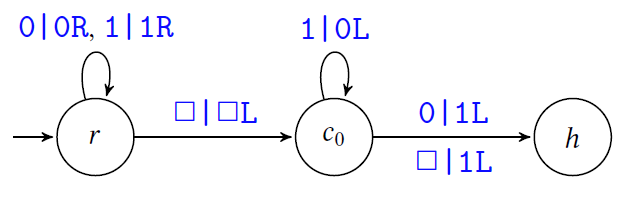
\includegraphics[scale=0.65]{turing/addBin1}
	\begin{center}
		\begin{tikzpicture}[->,>=stealth,shorten >=1pt,auto,node distance=2.8cm,
		semithick,initial text={}]
		\tikzstyle{every state}=[]
		
		\node[initial,state] (R)                    {$r$};
		\node[state]         (C) [right of=R] 	    {$c_0$};
		\node[state]         (H) [right of=C] 	    {$h$};
		
		\path 
		(R) edge [loop above] node {$\word 0\io\word 0R, \word 1\io\word1R$} (R)
		edge 					  node {$\9\io\9L$} (C)
		(C) edge [loop above] node {$\word 1\io\word 0L$} (C)
		edge 					  node {$\stackedtight{\word 0\io\word 1L, \\ \9\io\word 1L }$} (H)
		;
		\end{tikzpicture}
	\end{center}
	
	\smallskip
	\visible<2|handout:2>{
		Inkrementieren der dargestellten Zahl um $1$.
	}
\end{frame}

\begin{frame}{Aufgabe}
	Entwerft eine Turingmaschine, die für eine Eingabe $w \in \{\word 0, \word 1\}^*$ $$\fRepr_2(\fNum_2(w) - 1)$$ berechnet. Ihr dürft davon ausgehen, dass $\fNum_2(w) > 0$ gilt.\\
	\visible<2-|handout:2->{
		\begin{center}
			\begin{tikzpicture}[->,>=stealth,shorten >=1pt,auto,node distance=2.8cm,
			semithick,initial text={}]
			\tikzstyle{every state}=[]
			
			\node[initial,state] (R)                    {$r$};
			\node[state]         (C) [right of=R] 	    {$c_0$};
			\node[state]         (H) [right of=C] 	    {$h$};
			
			\visible<4-|handout:3->{
				\node[state]         (Z) [below=1cm of H] 	    {$z$};
			}
			\visible<6-|handout:4->{
				\node[state]         (L) [below=1cm of C] 	    {$\ell$};
			}
			
			\path 
			(R) edge [loop above] node {$\word 0\io\word 0R, \word 1\io\word1R$} (R)
			edge 					  node {$\9\io\9L$} (C)
			(C) edge [loop above] node {$\word 0\io\word 1L$} (C)
			edge 					  node {$\word 1\io\word 0L$} (H);
			
			\visible<4-|handout:3->{
				\path
				(H) edge [loop above] node {$\word 0\io\word 0L, \word 1\io\word1L$} (H)
				edge [left]				  node {$\9\io\9R$} (Z)
				(Z)  edge [loop right] node {$\word 0\io\9R$} (Z);
			}
			
			\visible<6-|handout:4->{
				\path
				(Z)  edge 				 node[below] {$\9\io\word 0L$} (L);
			}
			\end{tikzpicture}
		\end{center}
	}
	\visible<3-|handout:3->{\§{\textbf{Achtung}:} Was passiert mit führenden Nullen?} \\ 
	\visible<5-|handout:4->{\. Was, wenn es nur eine \word 0 gibt?} \\	
\end{frame}

\begin{frame}{Aufgabe}
	Wie würde man eine (einfache, nicht effiziente) TM zum Addieren von zwei Zahlen in Binärdarstellung aufbauen? \\ \pause
	\smallskip
	\impl Inkrementiere erste Zahl, dekrementiere zweite Zahl. Wiederhole, bis zweite Zahl $= 0$.
\end{frame}

\def\bword#1{\texttt{#1}}
\begin{frame}[t]{TM-Akzeptoren}
	\only<all:1>{
		Erinnerung: Inkrementieren um eins 
		\begin{center}
			\begin{tikzpicture}[->,>=stealth,shorten >=1pt,auto,node distance=2.8cm,
				semithick,initial text={}]
				\tikzstyle{every state}=[]
				
				\node[initial,state] (R)                    {$r$};
				\node[state]         (C) [right of=R] 	    {$c_0$};
				\node[state]         (H) [right of=C] 	    {$h$};
				
				\node[state,accepting,white]         (A) [below of=H] 	    {\phantom{$a_1$}};
				\node[state,white]         (B) [below of=C] 	    {\phantom{$a_2$}};
				
				\path 
				(R) edge [loop above] node {$\word 0\io\word 0R, \word 1\io\word 1R$} (R)
				edge 					  node {$\9\io\9L$} (C)
				(C) edge [loop above] node {$\word 1\io\word 0L$} (C)
				edge 					  node {$\stackedtight{\word 0\io\word 1L \\ \9\io\word 1L}$} (H)
				
				(H) edge [loop above,white] node {\phantom{$\word 0\io\word 0L, \word 1\io\word 1L$}} (H)
				(A)  edge [white]				 node[below] {\phantom{$\word 0\io\word 0L$}} (B)
				;
			\end{tikzpicture}
		\end{center}
	\mbox{}\vphantom{Welche Sprache....} \\
	}
	\only<all:2->{
		\?> TM-Akzeptor: 
		\begin{center}
			\begin{tikzpicture}[->,>=stealth,shorten >=1pt,auto,node distance=2.8cm,
				semithick,initial text={},every initial by arrow/.style={gray}]
				\tikzstyle{every state}=[]
				
				\node[initial,state,gray] (R)                    {$r$};
				\node[state,gray]         (C) [right of=R] 	    {$c_0$};
				\node[state]         (H) [right of=C] 	    {$h$};
				
				\node[state,accepting]         (A) [below of=H] 	    {$a_1$};
				\node[state]         (B) [below of=C] 	    {$a_2$};
				
				\path 
				(R) edge [loop above,gray] node {$\bword 0\io\bword 0R, \bword 1\io\bword 1R$} (R)
				edge [gray] 					  node {$\9\io\9L$} (C)
				(C) edge [loop above,gray] node {$\bword 1\io\bword 0L$} (C)
				edge [gray] 					  node {$\stackedtight{\bword 0\io\bword 1L \\ \9\io\bword 1L}$} (H)
				
				(H) edge [loop above] node {$\word 0\io\word 0L, \word 1\io\word 1L$} (H)
				edge [left]				  node {$\9\io\9R$} (A)
				(A)  edge [loop above left] node[left] {$\word 1\io\word 1R$} (A)
				(A)  edge 				 node[below] {$\word 0\io\word 0R$} (B)
				;
			\end{tikzpicture}
		\end{center}
		Welche Sprache akzeptiert diese TM? \\
	}
	\medskip
	\visible<3-|handout:2->{$\impl L(T) = \set{w \in \set{\word 0,\word 1}^* \Mid \fRepr_2(\fNum_2(w) + 1) \in \set{\word 1}^*}$}
\end{frame}

\begin{frame}{Turing-Maschinen vs. Supercomputer}
	Eine TM kann \textbf{genauso viel} berechnen wie euer Handy oder ein Supercomputer von Intel. {\small (Bloß halt etwas langsamer und umständlicher!)} \\
	\medskip
	Es gibt kein „mächtigeres“ Maschinenmodell als Turingmaschinen. \\
	\only<beamer:0>{
		\medskip 
		\begin{center}
			\impl Was eine Turingmaschine nicht berechnen \\ kann, kann keiner berechnen. \smiley \\ \#Prädikatenlogik-Blatt 2017/18
		\end{center}
	}
\end{frame}

\mycomment{ % Formalkram ist bähhh...
	% Ja, aber eigentlich wichtig. Aber dieses Jahr keine Zeit.
	\begin{frame}{Konfiguration}
		\begin{Definition}
			Als \textbf{Konfiguration} $ c =(z,b,p)$ bezeichnen wir den Zustand einer Turing-Maschine zu einem Zeitpunkt. Dabei ist 
			\begin{itemize}
				\item $z\in Z$ der Zustand
				\item $b: \Z\to X$ die Bandbeschriftung
				\item $p\in \Z$ die Position des Zeigers.
			\end{itemize}
		\end{Definition}
	\end{frame}
	
	\begin{frame}{Berechnungsschritte}
		\begin{Definition}
			In einem Berechnungsschritt geht eine TM aus einer Konfiguration $c$ 
			in die Konfiguration $$\Delta_1(c) := c' = (z',b',p')$$ über, wobei gilt:
			\begin{itemize}[<+->]
				\item $z' = f(z,b(p))$
				\item $\forall i\in \Z: b'(i) =
				\begin{cases}
				b(i) & \text{ falls } i\not=p \\
				g(z,b(p)) & \text{ falls } i=p
				\end{cases}$
				\item $p' = p + m(z,b(p))$
			\end{itemize}
			\bigskip
			
			\pause
			Wenn $\Delta_1(c)$ nicht definiert ist, bezeichnet man $c$ als \textbf{Endkonfiguration} und die TM \textbf{hält}.
		\end{Definition}
	\end{frame}
	
	\begin{frame}{Berechnungen}
		\begin{Definition}
			Eine Berechnung ist eine Folge von Konfigurationen $(c_0, c_1, ..., c_t)$ bei der gilt $$c_{i+1} = \Delta_1(c_i)$$ \pause
			Es gibt endliche, haltende (endet in einer Endkonfiguration) und unendliche Berechnungen.
			\bigskip
			
			\pause
			Induktiv definiert man $\Delta_t(c) , t\in\N_0$ als die Konfiguration, welche nach $t$ Berechnungsschritten erreicht werden kann und $\Delta_*(c)$ als Endkonfiguration, die von $c$ aus erreicht wird (falls die Berechnung endet).
		\end{Definition}
	\end{frame}
}








\begin{frame}{Entscheidbarkeit}
	\begin{Definition}
		Eine Sprache $L$ ist eine   
		\begin{itemize}[<+->]
			\item \textbf{aufzählbare Sprache}, wenn es eine Turingmaschine gibt, die $L$ akzeptiert.
			\item \textbf{entscheidbare Sprache}, wenn es eine Turingmaschine gibt, die $L$ akzeptiert und \emph{für jede Eingabe} hält.
		\end{itemize}
	\end{Definition} \pause
	
	Bei aufzählbaren Sprachen ist nicht definiert, wie sich die TM für Wörter $ w \notin L$ verhält. Sie kann diese ablehnen oder nicht halten. Ob eine TM für eine Eingabe nicht hält, können wir \enquote{von außen} nicht einfach feststellen.
\end{frame}


\begin{frame}{Aufgabe}
	Entwerft eine Turingmaschine, die die Sprache $ \{\word 0^k\word 1^k \mid k\in \N_0 \} $ akzeptiert.
	% TODO Lösung
\end{frame}

\begin{frame}{Aufgabe}
	Entwerft eine TM, die alle gültigen Klammerausdrücke entscheidet.\\
	\medskip
	Gültige Klammerausdrücke werden dabei von der folgenden Grammatik produziert: $ G = (\{S\},\{\word (, \word )\}, S, P )$ mit den Produktionen $\set{ S \to \eps \mid \word (S\word )S}$.
	% TODO Lösung
\end{frame}


\section{Komplexität}

\subsection{Unentscheidbare Probleme}
\begin{frame}{Unentscheidbare Probleme}
	Es existieren Probleme, die von keiner Turingmaschine entschieden werden können.\\ \pause
	\textbf{Erinnerung}: Entscheidbar heißt, dass es eine Turingmaschine gibt, die für jede Eingabe hält und entscheiden kann, ob das Wort in der Sprache liegt oder nicht. Statt \textbf{Sprachen} spricht man auch gerne von \textbf{Problemen}.\\ \pause
	
	\bigskip
	\textbf{Achtung}: Unentscheidbar meint wirklich \enquote{hält für manche Eingaben nie} und nicht \enquote{braucht $2^{2^{2^{n}}}$ Zeit}.
\end{frame}

\begin{frame}{Das Halteproblem}
	Im Folgenden: Turingmaschine $\equiv$ Java-Programm. {\small (Beide können genauso viel.)}\\ \pause
	\bigskip
	Als „Halteproblem“ bezeichnen wir salopp die Sprache aller haltenden Java-Programme.
	\begin{Definition} 
		\vspace{-1.5\baselineskip}
		\begin{align*}
		\text{Halteproblem } H &:= \set{w \in \set{\word 0, \word 1}^* \Mid w \text{ \textbf{beschreibt Turingmaschine}, die hält!}} \\
		&\:\approx \set{w \in \text{Java-Programme} \Mid w \text{ hält}} \\
		&\:\approx \set{w \in \text{C++-Programme} \Mid w \text{ hält}}
		\end{align*}
		Diese Definition ist ungenau, damit es nicht zu kompliziert wird. \textbf{Die offizielle Definition aus der VL ist allerdings wichtig!}
	\end{Definition}
\end{frame}

\mycomment{ % Viel zu kompliziert zum Vorziehen und sowieso keine Zeit dafür gehabt.
	% Falls irgendwann mal Zeit dafür sein sollte, dann müsste man das ganze eher visuell angehen oder wirklich die TGI-Version nehmen.
	\begin{frame}{Codierung von Turingmaschinen}
		In der VL: Codierung einer Turingmaschine als Wort über dem Alphabet \nolinebreak $\{0,1,[,]\} \qquad$ (Gödelisierung)
		\bigskip
		
		\begin{Satz}
			Es existiert eine universelle Turingmaschine $U$, die für zwei Eingaben $[\mathtt w_1][\mathtt w_2]$ 
			\begin{itemize}
				\item überprüft ob $\mathtt w_1$ eine Turingmaschine $T$ codiert
				\item falls ja, die Eingabe $\mathtt w_2$ auf dieser Turingmaschine simuliert
				\item Das Ergebnis davon berechnet (falls $T$ hält)
			\end{itemize}
		\end{Satz}
	\end{frame}
	
	\begin{frame}{Halteproblem}
		\begin{Satz}
			Es ist nicht möglich, eine Turingmaschine $H$ zu bauen, die für jede Turingmaschine $T$ und jede Eingabe $w$ entscheidet, ob $T$ bei der Eingabe von $w$ hält.
		\end{Satz}
	\end{frame}
	
	\begin{frame}{Beweis}
		Sei eine Tabelle $x_i, f_j$ gegeben, wobei die $x_i$ alle Codierungen einer Turingmaschine sind und die $f_j$ die berechneten Funktionen der Turingmaschine $T_j$ sind. Sei jetzt $H$ eine TM, die das Halteproblem löst und $G$ eine Maschine, die \begin{itemize}
			\item Wenn $H$ mitteilt, dass $T_{x_i} ( x_i )$ hält, dann geht $G$ in eine Endlosschleife.
			\item Wenn $H$ mitteilt, dass $T_{x_i} ( x_i )$ nicht hält, dann hält $G$
		\end{itemize}
		Jede mögliche Turingmaschine $T_{x_i}$ verhält sich also für die Eingabe $x_i$ genau anders wie $G$. Also ist $G$ eine Turingmaschine, die nicht in der Tabelle liegt, aber in der Tabelle sind alle TMs enthalten, da diese ja abzählbar sind. Widerspruch!
	\end{frame}
	
	\begin{frame}{Beweis 2}
		Sei wieder $H$ eine TM, die das Halteproblem löst und $G$ eine Maschine, die \begin{itemize}
			\item Wenn $H$ mitteilt, dass $T_{x_i} ( x_i )$ hält, dann geht $G$ in eine Endlosschleife.
			\item Wenn $H$ mitteilt, dass $T_{x_i} ( x_i )$ nicht hält, dann hält $G$
		\end{itemize}
		Also gilt: $$ G \text{ hält für Eingabe } w \iff T_w \text{ hält nicht für Eingabe } w $$
		Setzen wir nun für $w$ die Codierung von $G$ ein, so erhalten wir:
		$$ G \text{ hält für Eingabe } w \iff G \text{ hält nicht für Eingabe } w $$
		Widerspruch!
	\end{frame}
}

\begin{frame}{Das Halteproblem}
	\begin{Satz}
		Das Halteproblem ist unentscheidbar. \\
		Beweis: VL.
	\end{Satz}
	Das heißt, es kann \textbf{keine Turingmaschine} gebaut werden, die für jedes Java-Programm sagen kann, ob es hält oder nicht und dabei \textbf{selbst immer eine Antwort liefert}, also hält. \\ 
	\medskip \pause
	Es kann auch kein Java-Programm gebaut werden, welches das tut.
\end{frame}

\begin{headframe}
	\alert{\Huge Das HALTEPROBLEM ist unentscheidbar!}
\end{headframe}

\begin{headframe}
	\alert{\Huge Es gibt Probleme, die mit dem Rechner NICHT gelöst werden können!}
\end{headframe}

\begin{frame}{Fleißige Biber}
	\begin{Definition}
		Eine Bibermaschine ist eine Turingmaschine, die $n+1$ Zustände hat (wobei ein Anfangszustand und ein Haltezustand darunter sind) und die nur \word 1en produzieren kann.
	\end{Definition}
	\pause
	
	\begin{Definition}
		Als Busy-Beaver-Funktion $\bb(n)$ wird die maximale Anzahl an \word 1en bezeichnet, die ein Biber mit $n+1$ Zuständen auf dem Band hinterlassen kann. \\
		Ein Biber, der diese Zahl schafft, heißt auch \emph{fleißiger} Biber.
	\end{Definition} 
	
	\begin{Satz}
		Die Busy-Beaver-Funktion ist nicht berechenbar (es gibt keine Turingmaschine, die die Funktionswerte als Ausgabe liefert).
	\end{Satz}
\end{frame}

\begin{frame}[plain] \large \bf \centering
	Wir betrachten für die kommenden Folien nur Turingmaschinen, die bei jedem Eingabewort halten!
\end{frame}

\subsection{Berechnungskomplexität}
\begin{frame}{Zeitkomplexität}
	\textbf{Schaut euch das auch nochmal in der VL an!}
	\begin{Definition}
		Die Zeitkomplexität Time$(n)$ einer Turingmaschine ist die maximale Anzahl an Schritten, die eine Turingmaschine bei Eingabe eines Worts der Länge $n$ benötigen kann (worst-case).
	\end{Definition}
	\pause
	\textbf{Beispiel:} Überprüfung auf Palindrom:
	\begin{itemize}[<+->]
		\item Erstes Symbol \?> letztes Symbol ($n$) 
		\item Zurück zum ersten ($n$)
		\item Mit kürzerem Wort wiederholen ($n-2$)
	\end{itemize} \pause
	Also insgesamt $$\|Time|(n) \leq 2n + 1 + \|Time|(n-2)$$ 
	Daraus folgern wir $$\|Time|(n) \in O(n^2)$$
\end{frame}

\begin{frame}{Platzkomplexität}
	\begin{Definition}
		Die Platzkomplexität Space$(n)$ einer Turingmaschine ist die maximale Anzahl an Feldern, die eine Turingmaschine bei Eingabe eines Worts der Länge $n$ benötigen kann (worst-case). Benötigt wird ein Feld, wenn es vom Schreibkopf besucht wird oder von der Eingabe belegt wurde.
	\end{Definition}
	\pause
	\textbf{Beispiel:} Überprüfung auf Palindrom:
	\begin{itemize}[<+->]
		\item Erstes Symbol \?> letztes Symbol ($n + 1$) 
		\item Zurück zum ersten ($0$)
		\item Mit kürzerem Wort wiederholen ($0$)
	\end{itemize} \pause
	Also insgesamt $$\|Space|(n) = n+1 \in \Th{n}$$
\end{frame}

\begin{frame}{Platzkomplexität}
	Wie hängen Zeit- und Platzkomplexität zusammen?
	\begin{itemize}
		\item Wenn eine TM nur $n$ Schritte macht, kann sie auch nur $n$ Felder besuchen
		\item Aber anders herum: Auch mit $n$ Feldern können exponentiell viele Schritte durchgeführt werden.\\
			  Beispiel: Band mit $\word 0^n$. Solange inkrementieren (siehe Aufgabe), bis $\word 1^n$ auf dem Band steht. \pause Also $2^n - 1$ mal inkrementieren, somit mindestens $2^n - 1$ Schritte.
	\end{itemize}
\end{frame}

\begin{frame}
	\begin{Definition}
	\begin{itemize}
		\item \textbf{P} ist die Menge aller Entscheidungsprobleme, die von Turingmaschinen entschieden werden können, deren Zeitkomplexität polynomiell ist.
		\item \textbf{PSPACE} ist die Menge aller Entscheidungsprobleme, die von Turingmaschinen entschieden werden können, deren Raumkomplexität polynomiell ist.
	\end{itemize}
	\end{Definition}
	\pause
	Es ist \\ 
	\mbox{}\hphantom{Wir wissen nicht, ob auch \qquad }$\textbf{P} \subseteq \textbf{PSPACE}.$ \\
	\medskip\pause
	Die andere Richtung ist \textbf{ein großes offenes Problem}:\\
	Wir wissen nicht, ob auch \qquad $\textbf{P} \supseteq \PSPACE$. \\
	Wir haben zwar ein Beispiel für eine TM mit polynomiellen Platz und exponentieller Zeit gesehen, aber das \textbf{Problem} (alle $\word 0$ zu $\word 1$ umwandeln) hätte man deutlich effizienter lösen können.
\end{frame}

\subsection{Aufgabe}
\begin{frame}{Aufgabe} %(WS 2011)
	\only<1|handout:1>{	
		Die Turingmaschine $T$ mit Anfangszustand $S$ sei durch folgende Überführungsfunktion gegeben 
		\begin{table}[H]
		\centering
		\begin{tabular}{c|c|c|c|c}
		& $S$ & $S_a$ & $S_b$ & $R$ \\
		\hline
		$\word a$ & $(\word X,S_a,L)$ & $(\word a,S_a,L)$ & $(\word a,S_b,L)$ & $(\word a,R,R)$\\
		$\word b$ & $(\word X,S_b,L)$ & $(\word b,S_a,L)$ & $(\word b,S_b,L)$ & $(\word b,R,R)$\\
		$\word X$ & $(\word X,S,R)$ & $(\word X,S_a,L)$ & $(\word X,S_b,L)$ & $(\word X,S,R)$ \\
		$\square$ & --- & $(\word a,R,R)$ & $(\word b,R,R)$ & ---
		\end{tabular} 
		\end{table}
		\smallskip
		
		Tipp: Manchmal hilft es, die TM zu zeichnen.
	}

	\begin{itemize}
		\item Was steht bei der Eingabe des Wortes $w\in \{\word a,\word b\}^*$ am Ende der Berechnung auf dem Band? \\
			\only<2|handout:2>{\emph{Lösung}: Am Ende steht das Wort $R(w)\word X^{\vert w \vert}$ auf dem Band, wobei $R(w)$ das Spiegelbild von $w$ ist.}
		\item Welche Platzkomplexität hat $T$?\\
			\only<3|handout:2>{\emph{Lösung}: Eingabe der Länge $n$: Platzbedarf ist $2n+1$}
		\item Geben Sie eine einfache Funktion $f:\N_0 \functionto \N_0$ an, so dass die Zeitkomplexität von $T$ in $\Theta(f(n))$ liegt.\\
			\only<4|handout:2>{\emph{Lösung}: Eingabe der Länge $n$: Zeitbedarf in $\Theta(n^2)$ \\}
	\end{itemize}
\end{frame}



% TODO: Aufgaben!


% No longer todo: Fix dirty hack in thwregex.sty, where I changed line 42 to print star in math-mode
% 		because otherwise the star was always raised in my config.
%	COmment(Daniel): Reverted your change. No problems whatsoever.
%		Use \rx everywhere

% Fuck you, Latex. In my algo tutorial slides, this isn't necessary. Why here then!?
\begin{frame}[t]
	\fakeframetitle{\only<2->{Grenzen endlicher Akzeptoren}}
	Gibt es einen endlichen Akzeptor $A$ mit $$L(A) = \set{ \word a^k\word b^k \Mid k\in \N_0 }?$$
	\pause
	Nein! Warum nicht? \visible<3->{Endliche Automaten können nicht unendlich weit „zählen“!}\\
	
	Gibt es einen endlichen Akzeptor, der alle gültigen Klammerausdrücke erkennt?\\ \pause
	Nein, aus dem selben Grund.
	\begin{figure}[H]
		\centering
		
\includegraphics[scale=0.5]{xkcd/tags_1144}
		{ {\url{https://www.xkcd.com/1144/}} }
	\end{figure}
	\pause
	Kontextfreie Grammatiken \enquote{können also mehr} als endliche Akzeptoren.\\
	Wir wollen nun ein \enquote{gleichmächtiges} Konzept zu Akzeptoren.
\end{frame}

\section{Reguläre Ausdrücke}
\subsection{Definition}

\begin{frame}{Disclaimer!}
	\begin{center}
		\Large
			\bfalert{\Huge ACHTUNG!} \\ \medskip
		
		Gemeint sind \textbf{NICHT} sog. \emph{Regular Expressions}, die ihr vllt. aus Programmiersprachen kennt! \\ \bigskip
		
		{\normalsize (Die sind ähnlich, aber eben nicht das gleiche.)}
	\end{center}
\end{frame}

\begin{frame}{Reguläre Ausdrücke} 
	Bislang: Beschreibung der Sprache $L$ eines endlichen Akzeptors aus einzelnen Mengen, Vereinigung, Konkatenation, \dots \\
	$$ L = (\set{\word{ab}} \cdot \set{\word c, \word d})^\ast \cup \set{\word e}$$
	\medskip \pause
	
	Jetzt: Ein Ausdruck $R$, um eine mit solchen Operationen \enquote{zusammengebaute} Sprache zu beschreiben.\\
	$$ R = \rx{(ab(c|d))*|e}$$
	
	Wir bezeichnen die von $R$ beschriebene Sprache mit $\lang{R}$. \: Hier also: $L = \lang{R}$.\\
	Eine Sprache, für die es einen beschreibenden regulären Ausdruck gibt, nennt man \textbf{regulär}.
\end{frame}

\begin{frame}{Reguläre Ausdrücke}
	Wir können uns reguläre Ausdrücke zusammenbauen aus
	\begin{itemize}
		\item \hstretchto{\q15uad}{dem leeren Ausdruck $\rx O$} $\lang{\rx{O}} = \emptyset$\pause
		\item \hstretchto{\q15uad}{den einzelnen Symbolen $x \in A$}  $\lang{x}=\{x\}$ \pause
		\item zwei regulären Ausdrücken $R_1$ und $R_2$ mit\\ 
			\hstretchto{\q8uad}{$\rx(R_1 R_2\rx)$} $\lang{R_1 R_2} = \lang{R_1} \cdot \lang{R_2}$\\
			\hstretchto{\q8uad}{$\rx(R_1\rx|R_2\rx)$} $\lang{R_1 \rx| R_2} = \lang{R_1} \cup \lang{R_2}$ \pause
		\item \hstretchto{\q8uad}{einem Stern $R\rx*$} $\lang{R\rx*} = \lang{R}^*$\pause
	\end{itemize} 
	Klammern dürfen nach den Klammerregeln weggelassen werden:\\
	Stern vor „Punkt“ {\small (in diesem Fall unsichtbar)} vor Strich.
\end{frame}

\begin{frame}{Sprache eines regulären Ausdrucks}
	\begin{Beispiel}
		\begin{itemize}
			\item $\lang{\rx{a}} = \{\word a\}$. \pause
			\item $\lang{\rx{ab}} = \lang{\rx{a}} \cdot \lang{\rx{b}} = \{\word a\word b\}$. \pause
			\item $\lang{\rx{a|b}} = \lang{\rx{a}}\cup\lang{\rx{b}} = \{\word a,\word b\}$. \pause
			\item $\lang{\rx{(a|b)*}} = \lang{\rx{a|b}}^* = \{\word a,\word b\}^*$. \pause
			\item $\lang{\rx{(a*b*)*}} = \lang{\rx{a*b*}}^* = \left(\lang{\rx{a*}}\lang{\rx{b*}}\right)^* 
			= \left(\lang{\word a}^*\lang{\word b}^*\right)^* = \left(\{\word a\}^* \* \{\word b\}^*\right)^*$\\
			$= \{\word a,\word b\}^*$.  
		\end{itemize}
	\end{Beispiel}
	\pause
	\begin{block}{Aufgabe}
		Gebt einen regulären Ausdruck $R$ an mit $\lang{R} = $  
		\begin{itemize}
			\item die Sprache aller binären Zweierpotenzen \\ \visible<+->{}
				  \visible<+-|handout:2>{\impl $R = \rx{0*10*}$}
			\item die Sprache aller geraden Binärzahlen \\
				  \visible<+-|handout:2>{\impl $R = \rx{(0|1)*0}$}
		\end{itemize}
	\end{block}
\end{frame}

\begin{frame}{Aufgabe: Reguläre Ausdrücke}
	In dieser Aufgabe geht es um die formalen Sprachen
	$$L_1 = \set{\word a^k \word b^m \Mid k, m \in \N_0 }, \qquad L_2 = \set{\word b^k \word a^m \Mid k, m \in \N_0 }.$$
	Gebt für jede der folgenden formalen Sprachen $L$ je einen regulären Ausdruck $R$ an mit $ \langle R \rangle = L$.
	\begin{itemize}
		\item $L = L_1 \cup L_2$ \\
			\visible<2-|handout:2>{$ \rx{a*b*|b*a*}$}
		\item $L = L_1 \cap L_2$ \\
			\visible<3-|handout:2>{$ \rx{a*|b*}$}
		\item $L = L_1\cdot L_2$ \\
			\visible<4-|handout:2>{$ \rx{a*b*b*a*}$ oder $\rx{a*b*a*}$}
		\item $L = L_1^*$ \\
			\visible<5-|handout:2>{$ \rx{(a*b*)*}$ oder $\rx{(a|b)*}$}
	\end{itemize}
\end{frame}

\begin{frame}{Aufgabe: Sprachen regulärer Ausdrücke}
	\begin{itemize}
		\item $\lang{\rx{(a|b)*abb(a|b)*}} = \visible<2-|handout:2>{\{\word a, \word b\}^* \cdot \{\word a\word b\word b\} \cdot \{\word a, \word b\}^*}$
		\item $\lang{\rx{a**}} = \visible<3-|handout:2>{\{\word a\}^*}$
		\item $\lang{\visible<4-|handout:2>{R\rx{(}R\rx{)*}}} = \lang{R}^+$ \quad (für bel. reg. Ausdruck $R$)
		%\item $\lang{\visible<5-|handout:2>{\rx{O*}}} = \{\eps\}$
		\item $\lang{\visible<5-|handout:2>{\rx{a*ba*ba*b(a|b)*}}} = \set{ w \in \{\word a, \word b\}^* \Mid \size{w}_{\word b} > 2 } $
		\item $\lang{\visible<6-|handout:2>{\rx{b*a*}}} =$ Sprache aller Wörter über $\set{\word a, \word b}$, in denen das Teilwort \word{ab} nicht vorkommt.
	\end{itemize}
\end{frame}


\input{../Bloecke/RechtslineareGrammatiken}

\begin{frame}{Turingmaschinen: Klausur}
	Noch ein Hinweis zum Schluss:\\
	Bisher kam in {\tiny fast} \textbf{jeder} Klausur eine Aufgabe zu Turingmaschinen dran.\\
	Diese gibt meist relativ viele Punkte.\\
	
	\bigskip
	Es ist hochwahrscheinlich, dass auch dieses Mal wieder eine TM-Aufgabe drankommt.\\
	\textbf{Also übt das!} Hier zählt vor allem Geschwindigkeit (und Präzision).
\end{frame}

\begin{frame}	
	\begin{block}{Was ihr nun wissen solltet}
		\begin{itemize}
			\item Turingmaschinen
			\item Komplexität
			\item Entscheidbarkeit -- Wir können alles. Außer Halteproblem. Und so Zeug.
			\item Reguläre Ausdrücke
			\item Rechtslineare Grammatiken
		\end{itemize}
	\end{block}
	
	%\begin{block}{Was nächstes Mal kommt}
	%	\begin{itemize}
	%		\item Reguläre Ausdrücke
	%		\item Rechtslineare Grammatiken
	%	\end{itemize}
	%\end{block}
\end{frame}

% TODO ?
%input{../Bloecke/StrukturelleInduktion}

%TODO replacement?
{\xkcdframe{1724}{Danke für eure Aufmerksamkeit! \smiley}{2.5}}
%\thasse{\lastframe{0.5}{0}{xkcd/proofs_1724.png}{https://www.xkcd.com/1724/}}

\slideThanks

\end{document}